\subsection{Learning from event counts and selecting a certified policy}
The reserve experiment tests the partially observed simulator with a specified latent model. A separate finite observable example tests the statistical and control results of \Cref{sec:certified-control} using event data alone. Its role is to isolate what can be certified when state-action exposure is actually observed.

The state is $(q,z)$ with remaining quantity $q\in\{0,1,2,3,4\}$ and observed regime $z\in\{0,1\}$. The actions are passive ($a=0$) and aggressive ($a=1$). A fill reduces $q$ by one; a regime mark changes $z$ to $1-z$. States with $q=0$ are absorbing. For positive quantity the synthetic rates are
\begin{align}\label{eq:control-truth}
 \lambda_{\rm fill}(q,z,a)&=(0.75+0.10q)(1+0.35z)(1+1.8a),\\
 \lambda_{\rm regime}(q,z,a)&=0.35+0.10q+0.12a+0.20z.\notag
\end{align}
Their known envelopes are $5$ and $1.5$. At horizon $T=2$, the terminal cost is $q(1+0.2z)$; running cost is $0.03q^2$; a passive fill costs $0.03$ and an aggressive fill costs $0.35$. Regime changes have no direct cost. This fully specified objective measures an execution trade-off, without purporting to reproduce an exchange fee schedule or empirical spread process.

Each observed episode starts with randomized positive quantity and regime. A behavior action is chosen independently at the initial state and after each event, and held until the next event or horizon. The recorded sufficient statistics are the event counts and occupation times for every state-action-mark triple. Three independent streams use seeds $5101,5102,5103$ and prefixes of $2{,}000$, $8{,}000$, and $32{,}000$ episodes. The rate intervals use sixteen geometrically spaced positive $\eta$ values between $0.005$ and $1$, with the 1\% failure budget divided across the three streams. Time-uniform coverage includes every prefix without an additional prefix penalty. The 32 active triples, confidence endpoints, exposures, and counts are serialized.

A $3\to12\to2$ tanh network with sigmoid rate outputs has 74 parameters. Its inputs encode quantity, regime, and action, and its output envelopes are the known rate caps. Training uses $1{,}400$ Adam steps on the exposure-weighted negative log-likelihood
$\sum_i\{\widehat\lambda_i E_i-N_i\log\widehat\lambda_i\}$.
The true rates in \eqref{eq:control-truth} are never training labels. The deployed rate vector is clipped to the confidence box, with the raw network output also retained. The nominal neural policy minimizes its estimated cost. The robust policy minimizes the upper Hamiltonian over the whole box; its guarantee does not depend on successful network optimization. This separation makes it possible to assess both learned predictions and uncertainty-aware decisions.

Both robust equations use $8{,}000$ time steps and the residual allowance in \Cref{prop:control-residual}. The true costs of the resulting feedback policies are computed by matrix exponentiation over runs of identical action vectors. This evaluates the actual continuous-time policy, including possible changes of action at grid boundaries. A high-accuracy DOP853 solution computes the known-model optimum, independently cross-checked against a $16{,}000$-step Euler solution and its residual allowance. Truth enters these diagnostics, not the data-derived confidence box or robust decision.

\begin{table}[htbp]
\centering\small
\begin{tabular}{rrrrr}
\toprule
Episodes & Neural regret & Robust regret & 99\% regret bound & Time residual \\
\midrule
2,000 & 0.00214 & 0.02138 & 1.0618 & 0.0104 \\
8,000 & 0.00014 & 0.00657 & 0.4681 & 0.0105 \\
32,000 & 0.00004 & 0.00161 & 0.2341 & 0.0102 \\
\bottomrule
\end{tabular}

\caption{Execution from initial state $(4,0)$. The neural and robust regrets are means over the three fixed data streams, evaluated against the known synthetic optimum. The confidence column is the largest theorem-derived bound across those streams, including time discretization; the final column is the largest sum of numerical residual allowances. Confidence refers to the analytic event, not a formally rounded floating-point enclosure.}\label{tab:certified-control}
\end{table}

The known optimum is $1.733392$. At $32{,}000$ episodes, robust-policy regret ranges from $0.001178$ to $0.001968$, while its certificate ranges from $0.226235$ to $0.234137$. All true rates fall inside their intervals in the reported runs; this observed coverage is a diagnostic, not a substitute for the simultaneous theorem. The nominal neural policy has lower realized regret in these examples. Robustness therefore has a measured conservatism cost; these experiments do not claim that pessimism always improves realized performance. Rectangular uncertainty and protection against every admissible rate vector explain part of the gap between measured regret and its bound.

\begin{figure}[htbp]
\centering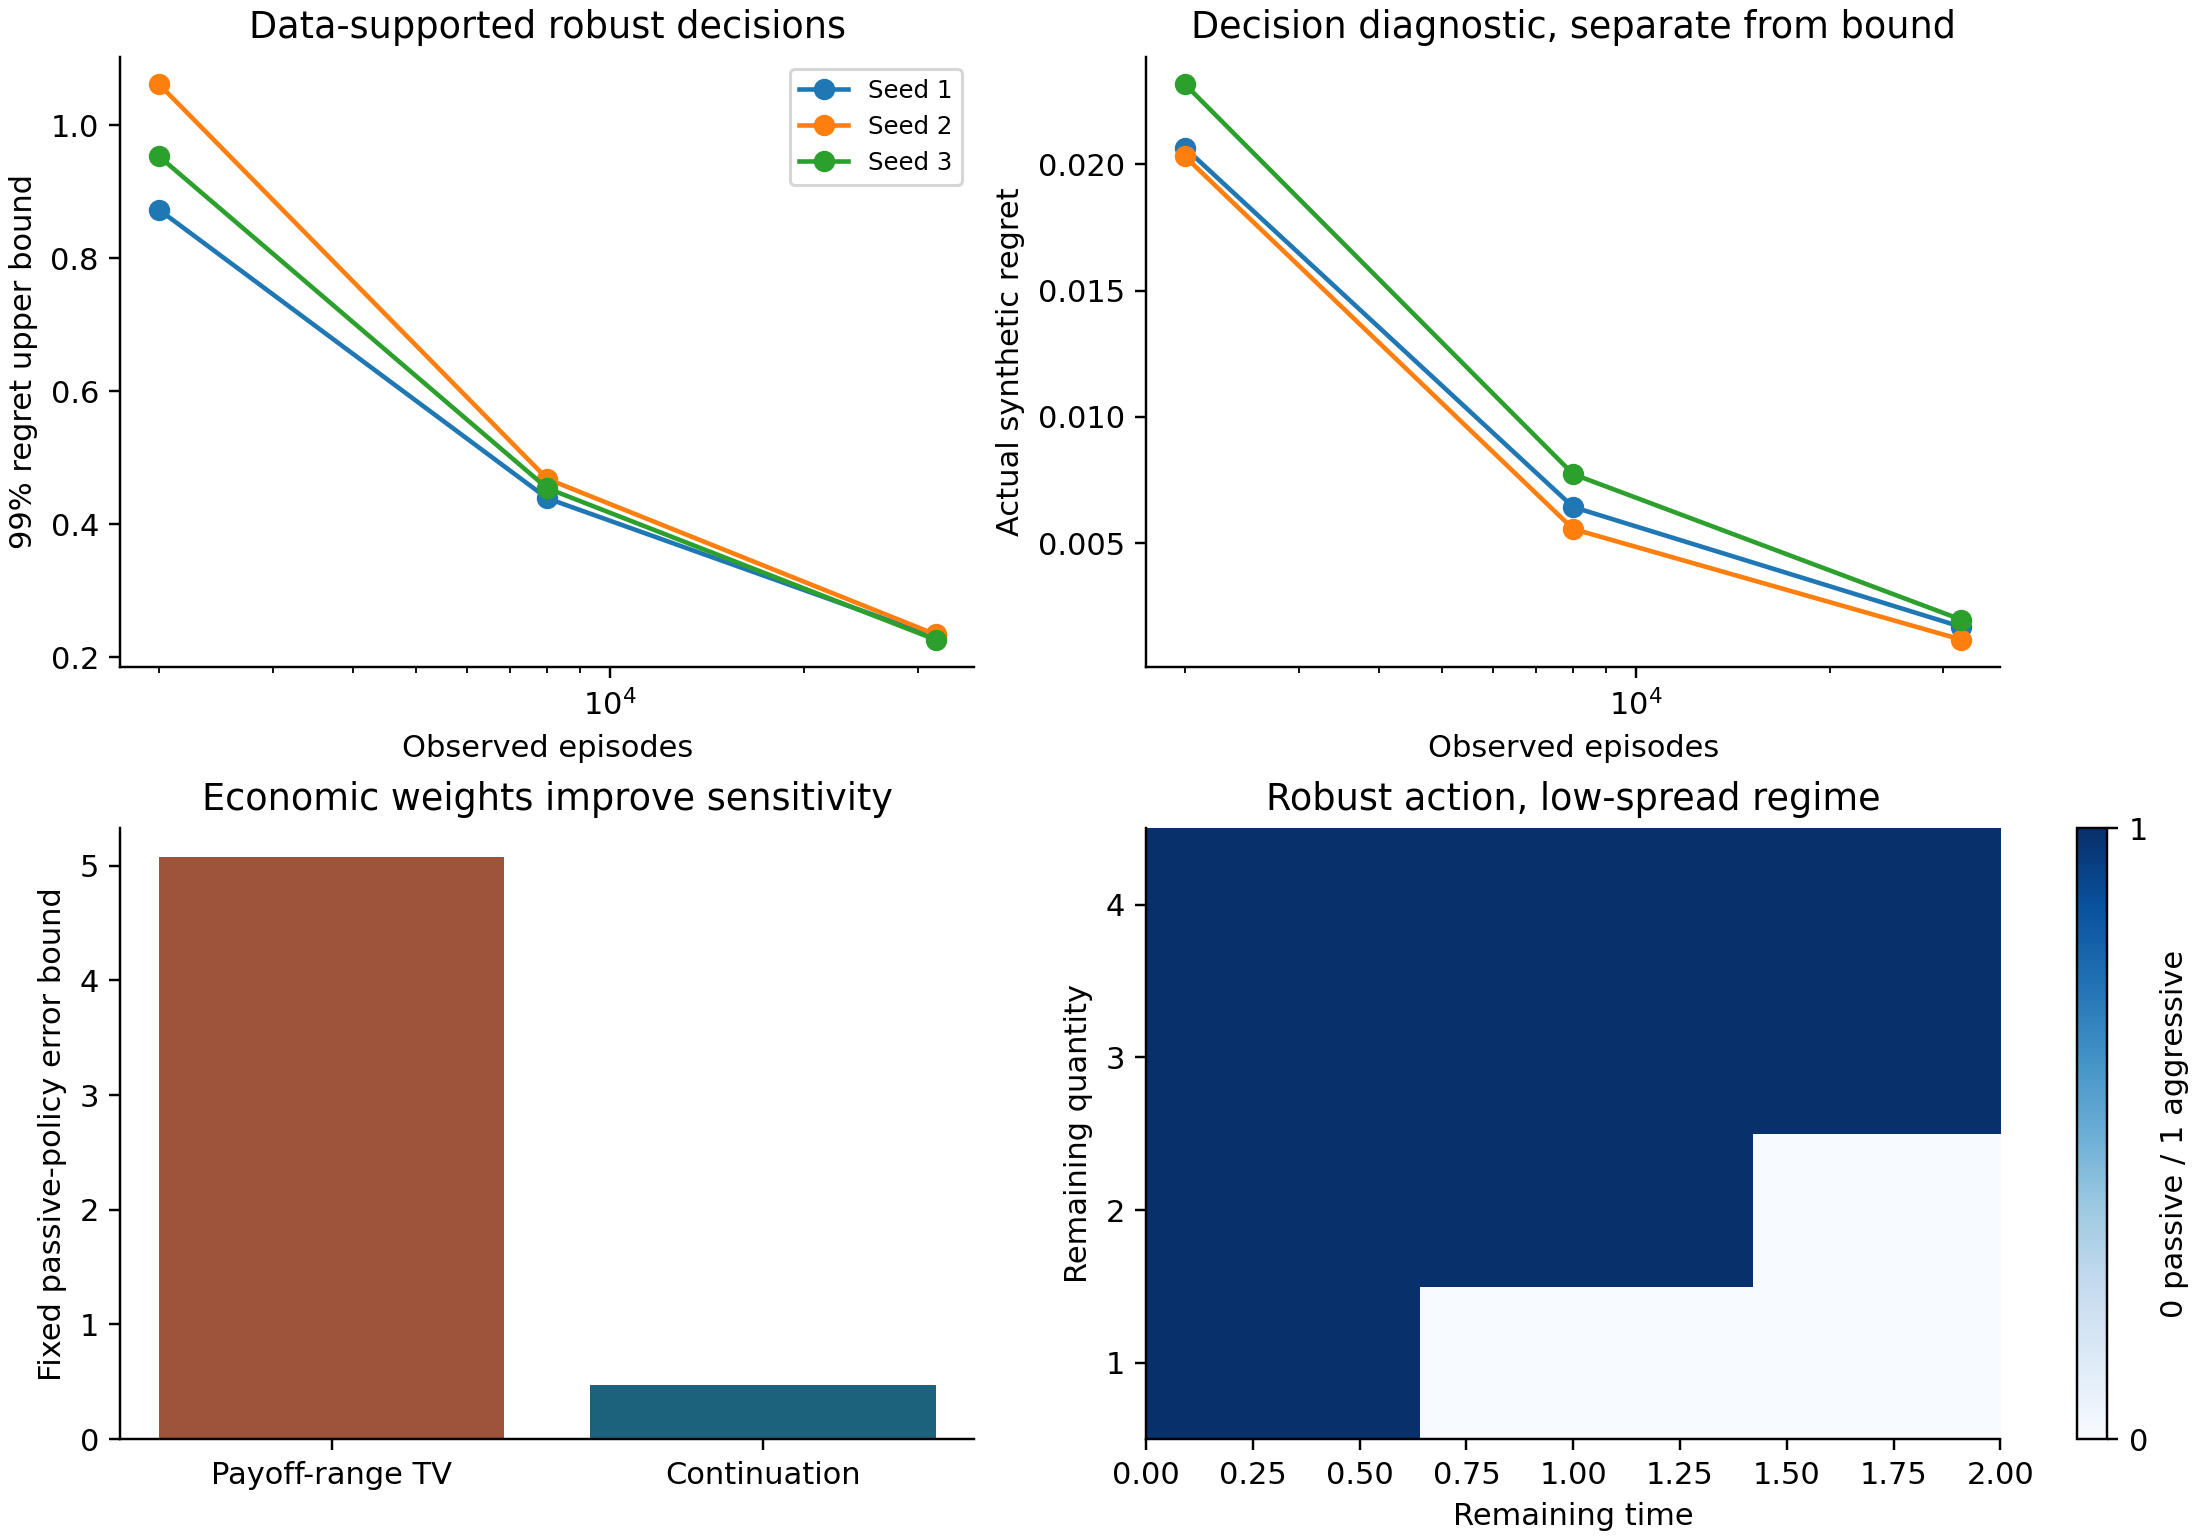
\includegraphics[width=\textwidth]{figures/certified_control.png}
\caption{Observed-event learning and decision certification. Upper panels separate the simultaneous regret bound from actual synthetic regret. Lower left compares two uncertainty bounds for a fixed passive policy. Lower right shows the robust feedback action at the largest data budget of the first stream.}\label{fig:certified-control}
\end{figure}

\subsection{Sensitivity and numerical error in the same decision model}
For the fixed passive policy in the first stream's largest dataset, the exact true-minus-learned cost difference is $-0.00904582$. Numerical integration of the signed continuation identity differs by only $4.82\times10^{-9}$. The statewise continuation bound is $0.469600$, compared with $5.071310$ from the payoff-range times path-TV route using the same rate intervals. Their ratio is about $10.80$. The comparison is objective-specific; a different payoff can assign very different weights to the same events. The continuation integral is numerically evaluated on 2,001 time points and is not claimed to have a rigorous quadrature enclosure.

Doubling the upper-control grid from $8{,}000$ to $16{,}000$ steps changes its initial value by $7.32\times10^{-5}$. The corresponding analytic residual allowances are $0.004900$ and $0.002450$. This check supports the implementation and expected first-order refinement. The allowance bounds the continuous-time interpolation error in exact arithmetic; the program labels its floating-point results accordingly.

Finally, the equal-terminal-law example in \Cref{ex:early-information}, evaluated at $r=0.1$, has early-revelation American value $0.452419$ and late-revelation value $0.409365$. The European values coincide at $0.409365$. The calculation isolates information timing, which neither terminal-law calibration nor an arbitrary path coupling can remove.
